\documentclass[12pt,letterpaper,twoside]{article}
\usepackage{amsmath,amssymb,amsfonts}
\usepackage{graphicx}
\usepackage{tikz}
\usepackage{pgfplots}
\pgfplotsset{compat=1.17}
\usepackage{enumitem}
\usepackage{hyperref}
\usepackage{cleveref}
\usepackage{authblk}
\usepackage{caption}
\usepackage{subcaption}
\usepackage{xcolor}
\usepackage{geometry}
\geometry{margin=1in}

% Math commands
\newcommand{\R}{\mathbb{R}}
\newcommand{\T}{\mathbb{T}}
\newcommand{\C}{\mathbb{C}}
\newcommand{\N}{\mathbb{N}}
\newcommand{\Z}{\mathbb{Z}}
\newcommand{\Q}{\mathbb{Q}}
\newcommand{\id}{\mathrm{id}}
\newcommand{\diag}{\mathrm{diag}}
\DeclareMathOperator{\Diff}{Diff}
\DeclareMathOperator{\Exp}{Exp}
\DeclareMathOperator{\Log}{Log}
\DeclareMathOperator{\Ric}{Ric}
\DeclareMathOperator{\scal}{scal}
\DeclareMathOperator{\vol}{vol}

% Custom colors
\definecolor{manifoldblue}{RGB}{33, 97, 140}
\definecolor{manifoldred}{RGB}{180, 60, 60}
\definecolor{manifoldgreen}{RGB}{60, 140, 80}

% Title and author information
\title{The Hyper-Torus: Topology-Aligned Geometry for Constant-Memory Sequence Modeling}
\author{Joaquin Stürtz}
\date{January 24, 2026}
\affil{Independent Researcher}

\begin{document}
\maketitle

\begin{abstract}
Cyclic reasoning tasks (parity, modular arithmetic, periodic phase tracking) are poorly expressed in Euclidean latent spaces. We present the \textbf{Hyper-Torus}, a topology-aligned manifold design that embeds periodic structure natively into the latent geometry of sequence models. The Hyper-Torus is built from a product of circles $\T^d = S^1 \times S^1 \times \cdots \times S^1$ equipped with the standard product metric, providing natural periodicity without boundary artifacts or learned phase offsets. We demonstrate that models utilizing Hyper-Torus latents achieve superior performance on tasks requiring modular arithmetic, temporal pattern recognition, and long-range cyclic dependencies, while using substantially fewer parameters and maintaining constant memory overhead independent of sequence length. The topological alignment between model geometry and task structure yields interpretable latent representations and improved sample efficiency. Our framework provides a principled approach for incorporating periodic inductive biases into deep learning architectures.
\end{abstract}

\section{Introduction}
Sequence modeling forms the backbone of modern deep learning applications, encompassing natural language processing, time-series analysis, protein structure prediction, and reinforcement learning. Despite remarkable advances in transformer architectures and recurrent networks, a fundamental tension persists between model capacity and computational efficiency. Most state-of-the-art sequence models operate in Euclidean latent spaces $\R^d$, which, while mathematically convenient, impose strong inductive biases that may conflict with the inherent structure of many sequential tasks. In particular, \textbf{periodic phenomena}—tasks involving cycling, modular arithmetic, phase tracking, or temporal patterns—remain challenging for Euclidean models, which must learn to approximate periodic structure from data rather than having it built into their geometry.

Consider the task of counting parity: given a sequence of bits, the model must output the parity (even or odd) of the number of ones encountered. This task has an inherently cyclic nature, as adding two ones flips the parity twice, returning to the original state. Similarly, modular arithmetic operations such as addition modulo $n$ exhibit perfect periodicity, as do many temporal patterns in speech, music, and biological signals. Euclidean latent spaces lack native periodic structure, forcing models to approximate periodicity through complex learned transformations that introduce boundary artifacts at $\pm\infty$ and require careful initialization and regularization to function adequately.

The \textbf{Hyper-Torus} architecture addresses this fundamental limitation by replacing the Euclidean latent space with a compact manifold homeomorphic to a $d$-dimensional torus. A $d$-dimensional torus $\T^d$ is defined as the Cartesian product of $d$ circles: $\T^d = S^1 \times S^1 \times \cdots \times S^1$. Each circle $S^1$ can be parameterized by an angle $\theta \in [0, 2\pi)$, with the endpoints identified to create a smooth, compact manifold without boundaries. The product structure provides $d$ independent periodic directions, allowing the model to encode $d$ separate periodicities simultaneously while maintaining geometric coherence.

This paper makes the following contributions to the field of geometric deep learning for sequence modeling:

\begin{enumerate}[label=(\roman*)]
    \item We introduce the \textbf{Hyper-Torus} manifold, a principled geometric framework for incorporating periodic inductive biases into sequence models.
    \item We derive efficient algorithms for computing exponential and logarithmic maps on the product torus, enabling gradient-based optimization of points on the manifold.
    \item We develop a \textbf{Hyper-Torus Neural Network} architecture that processes sequences while maintaining latent representations on the torus, with constant memory overhead regardless of sequence length.
    \item We provide extensive experimental evidence demonstrating superior performance on periodic reasoning tasks compared to Euclidean baselines.
    \item We analyze the learned latent representations to demonstrate that the topology-aligned geometry yields interpretable and semantically meaningful encodings.
\end{enumerate}

The Hyper-Torus framework represents a significant step toward \textbf{topology-aware neural network design}, where the geometric structure of the latent space is chosen to align with the topological structure of the target task. This alignment provides both computational benefits—reducing the effective dimensionality of the learning problem—and statistical benefits—improving sample efficiency by reducing the hypothesis space to geometrically appropriate functions.

\section{Mathematical Foundations}
The mathematical foundation of the Hyper-Torus architecture rests on differential geometry, particularly the theory of Lie groups and homogeneous spaces. The $d$-dimensional torus $\T^d$ is a compact, connected, abelian Lie group with rich geometric structure that we leverage for sequence modeling.

The $n$-dimensional torus $\T^n$ is defined as the quotient space $\R^n / \Z^n$, where $\Z^n$ acts on $\R^n$ by integer translation. Equivalently, $\T^n$ can be realized as the product of $n$ circles: $\T^n = S^1 \times S^1 \times \cdots \times S^1$. Each circle $S^1$ can be embedded in $\R^2$ as the set $\{(\cos\theta, \sin\theta) : \theta \in [0, 2\pi)\}$, and the torus inherits the product metric from this embedding. The standard metric on $\T^n$ has constant sectional curvature zero, making it a flat manifold in the Riemannian sense.

\begin{remarque}[Reactive Metric Note]
While the canonical torus is flat, advanced GFN implementations (see Paper 02: Reactive Geometry) often employ a \textit{reactive metric} $g_{ij}(x,v)$ that introduces local curvature variations proportional to the kinetic energy of the latent state. This allows the manifold to ``stiffens'' in high-energy regions, stabilizing dynamics, while retaining the global topological properties of the flat torus.
\end{remarque}

The flatness of the torus has important implications for gradient-based optimization. Unlike positively curved manifolds such as spheres, where the exponential map contracts distances for large step sizes, the torus's flat geometry ensures that geodesic distances are proportional to the parameter differences throughout the entire manifold. This property simplifies training dynamics and eliminates the need for specialized retraction operators or geodesic optimization schemes that are necessary on curved manifolds.

The Lie group structure of $\T^n$ provides natural group operations that can be leveraged for sequence processing. Addition on the torus corresponds to component-wise addition modulo $2\pi$, enabling compositional operations that preserve the manifold structure. This group structure is particularly valuable for modeling sequences where operations should commute and be invertible—properties that are automatically satisfied on the torus but require careful architectural design in Euclidean spaces.

The topology of the torus fundamentally differs from that of Euclidean space. While $\R^n$ is contractible (it can be continuously deformed to a point), $\T^n$ has nontrivial first homology group $H_1(\T^n; \Z) \cong \Z^n$, reflecting the presence of $n$ independent non-contractible loops. This topological structure means that paths on the torus can wrap around the manifold multiple times, creating distinct homotopy classes that Euclidean space cannot distinguish. For periodic tasks, this topological richness aligns precisely with the structure of the problem.

The fundamental group $\pi_1(\T^n) \cong \Z^n$ classifies loops on the torus up to continuous deformation. Each element of $\Z^n$ corresponds to a loop that wraps around a specific collection of the $n$ circular factors a given number of times. For a parity task, the relevant topological feature is a loop that wraps around a single circle an odd number of times—the fundamental distinction between even and odd is precisely captured by the winding number in $\Z$.

When we embed periodic structure into a Euclidean latent space, we lose access to these topological invariants. A model operating in $\R^n$ cannot distinguish between a path that wraps around a circle an odd number of times and a path that wraps around it an even number of times, as both correspond to paths that start and end at the same point. The model must learn to detect periodicity through functional properties rather than having it available as a geometric primitive.

The flat metric on $\T^n$ has Riemann curvature tensor identically zero, making the torus a locally isometric copy of Euclidean space. However, the global topology creates interesting global phenomena—geodesics can be closed and multiple distinct geodesics can connect the same points, wrapping different numbers of times around the compact dimensions. This combination of local flatness and global structure is unique to the torus and provides both computational simplicity (local geometry is Euclidean) and topological richness (global structure is non-trivial).

For sequence modeling, we leverage the \textbf{product structure} of the torus. If our latent space is $\T^d$, we can allocate different circular dimensions to different periodic features in the data. For example, in a music modeling task, one dimension might encode the beat phase (period 1), another the measure phase (period 4), another the key cycle (period 12 for chromatic scale), and another the song form (period 32 measures). The product structure naturally separates these scales while allowing them to interact through the metric connection.

The logarithmic map on the torus is particularly simple: for two points $x, y \in \T^n$, the logarithmic map $\Log_x(y)$ returns the tangent vector at $x$ that generates $y$ via the exponential map. In coordinates, if $x = (x_1, \ldots, x_n)$ and $y = (y_1, \ldots, y_n)$ with each coordinate in $[0, 2\pi)$, then:
\begin{equation}
\Log_x(y)_i = \begin{cases}
y_i - x_i & \text{if } |y_i - x_i| \leq \pi \\
y_i - x_i - 2\pi & \text{if } y_i - x_i > \pi \\
y_i - x_i + 2\pi & \text{if } y_i - x_i < -\pi
\end{cases}
\end{equation}
This formula implements the ``shortest arc'' convention on each circle, ensuring that the logarithmic map returns the minimal tangent vector connecting the points. The exponential map is similarly straightforward, wrapping the tangent vector back onto the circle.

The injectivity radius of the torus is $\pi$, meaning that the exponential map is a diffeomorphism from the open ball of radius $\pi$ in $T_x\T^n$ onto its image. This bound is tight—a tangent vector of length $\pi$ in any direction produces a point antipodal to $x$ on the corresponding circle, and longer vectors would produce the same point through different winding numbers. In practice, gradient steps are typically much smaller than $\pi$, so the exponential map is locally well-behaved throughout training.

The volume of $\T^n$ with respect to the standard metric is $(2\pi)^n$, making it a compact manifold with finite total volume. This compactness has implications for probability distributions on the torus—any continuous distribution must assign positive probability density somewhere, and there is no ``out-of-distribution'' region at infinity. For sequence modeling, this means that latent representations remain bounded regardless of how long the sequence grows, preventing the unbounded drift that can occur in Euclidean latent spaces.

The spectral geometry of the torus is also well-understood. The Laplacian on $\T^n$ has eigenvalues and eigenfunctions given by products of sine and cosine functions on each circle, known as the Fourier basis. The eigenvalues are $\lambda_k = k_1^2 + k_2^2 + \cdots + k_n^2$ for $k \in \Z^n$, with multiplicity growing with the eigenvalue. This connection to Fourier analysis suggests that neural networks on the torus may have natural frequency-domain interpretations, which could be valuable for signal processing applications.

The Fourier perspective also illuminates the relationship between torus and Euclidean representations. Any square-integrable function on $\T^n$ admits a Fourier series expansion, and the Fourier modes form an orthonormal basis of $L^2(\T^n)$. The Fourier coefficients can be computed via integration over the torus, and the topology of the torus ensures that these coefficients capture all periodic structure in the function. In contrast, a Euclidean space $\R^n$ requires the more general Fourier transform, which produces a continuum of frequencies rather than a discrete spectrum.

For neural network design, the Fourier perspective suggests that convolution operations on the torus correspond to multiplication in Fourier space, just as in the Euclidean case. The main difference is that the torus convolution kernel must be periodic, which is automatically satisfied by restricting the kernel to the fundamental domain $[0, 2\pi)^n$. This suggests that convolutional architectures can be directly adapted to the torus setting with minimal modification.

The geodesic distance between two points $x, y \in \T^n$ is given by:
\begin{equation}
d(x, y) = \sqrt{\sum_{i=1}^n \min(|x_i - y_i|, 2\pi - |x_i - y_i|)^2}
\end{equation}
This distance is always well-defined and bounded by $\pi\sqrt{n}$, providing a natural measure of dissimilarity that respects the manifold topology. Unlike Euclidean distance, geodesic distance on the torus is periodic and handles the identification of endpoints gracefully.

The parallel transport on the torus is trivial: since the manifold is flat, parallel transport along any path preserves tangent vectors without rotation or holonomy. This means that gradient vectors computed in different tangent spaces can be compared and combined without accounting for curvature-induced rotations—a significant simplification compared to training on curved manifolds such as spheres or hyperbolic spaces.

In summary, the torus $\T^n$ provides a geometric space that is simultaneously:
\begin{itemize}
    \item \textbf{Compact}: All points are at bounded distance, preventing unbounded latent drift.
    \item \textbf{Flat}: Local geometry is Euclidean, simplifying gradient-based optimization.
    \item \textbf{Periodic}: Native support for periodic structure through circular topology.
    \item \textbf{Product}: Multiple independent periodicities can be represented simultaneously.
    \end{itemize}
These properties make the torus an ideal candidate for the latent space of sequence models dealing with periodic or cyclic phenomena.

\section{Constant-Memory Sequence Modeling}
The computational architecture of Hyper-Torus Networks builds upon the insights of section 2 to create a sequence model with constant memory overhead. The key observation is that the group structure of the torus enables compositional updates that do not require storing intermediate hidden states—each step's output depends only on the current latent state, not on the full history.

Consider a sequence of input tokens $x_1, x_2, \ldots, x_T$. In a standard recurrent neural network, the hidden state $h_t$ evolves according to $h_t = f(h_{t-1}, x_t)$, requiring storage of the entire sequence of hidden states for backpropagation through time. This creates linear memory overhead in the sequence length and introduces challenges for very long sequences due to gradient clipping requirements and vanishing/exploding gradient problems.

In a Hyper-Torus Network, the latent state $z_t$ lives on the torus $\T^d$. Updates proceed via group multiplication:
\begin{equation}
z_t = z_{t-1} \cdot \phi(x_t)
\end{equation}
where $\phi: \mathcal{X} \to \T^d$ is an embedding function mapping inputs to the torus, and $\cdot$ denotes the group operation (component-wise addition modulo $2\pi$). This update rule is \textbf{associative}: the state after processing the first $t$ tokens is $z_t = z_0 \cdot \phi(x_1) \cdot \phi(x_2) \cdot \cdots \cdot \phi(x_t)$, which depends only on the current state and the new input, not on the history of states.

The associativity of the group operation is crucial. It means that the update rule $z_t = z_{t-1} \cdot \phi(x_t)$ can be computed online without reference to earlier states. After processing $t-1$ tokens, we have $z_{t-1} = z_0 \cdot \phi(x_1) \cdot \cdots \cdot \phi(x_{t-1})$. Adding $x_t$ requires only the current state $z_{t-1}$ and the new contribution $\phi(x_t)$, not the intermediate products.

This property enables \textbf{constant-memory sequence processing}: regardless of sequence length, only the current latent state $z_t$ needs to be stored. The memory footprint is $O(d)$ for a $d$-dimensional torus, independent of $T$. This is in stark contrast to transformer architectures with $O(T^2)$ attention memory or RNNs with $O(T \cdot d)$ hidden state storage.

The associative structure also enables efficient gradient computation through backpropagation. The gradient of the loss $\mathcal{L}$ with respect to the input embeddings depends only on the final state and the loss gradient, not on the full sequence of hidden states. Using the adjoint method for optimal control, we can compute gradients in time linear in $T$ but with constant memory overhead.

Mathematically, let $z_t = z_{t-1} + \phi(x_t)$ denote the update (using additive notation for the torus group). The loss gradient backward pass computes:
\begin{align}
\frac{\partial \mathcal{L}}{\partial z_{t-1}} &= \frac{\partial \mathcal{L}}{\partial z_t} \frac{\partial z_t}{\partial z_{t-1}} = \frac{\partial \mathcal{L}}{\partial z_t} \\
\frac{\partial \mathcal{L}}{\partial \phi(x_t)} &= \frac{\partial \mathcal{L}}{\partial z_t} \frac{\partial z_t}{\partial \phi(x_t)} = \frac{\partial \mathcal{L}}{\partial z_t}
\end{align}
The Jacobian $\frac{\partial z_t}{\partial z_{t-1}}$ is the identity matrix, simplifying the backward pass considerably. Each step's gradient depends only on the gradient from the next step, enabling a backward pass that sweeps through the sequence once, maintaining only the current gradient value.

This gradient flow is markedly different from RNNs, where the Jacobian $\frac{\partial h_t}{\partial h_{t-1}}$ is typically a nontrivial matrix that can amplify or attenuate gradients exponentially in the sequence length. On the torus, the identity Jacobian eliminates these effects, providing stable gradient flow regardless of sequence length.

The constant-memory property extends to inference as well as training. At inference time, we only need to maintain the current latent state $z_t$ while processing the sequence token by token. This enables processing of arbitrarily long sequences on devices with limited memory, or streaming processing where sequences arrive continuously.

The computational complexity per token is $O(d^2)$ for matrix operations, or $O(d)$ if we use element-wise operations. This matches the per-step complexity of simple RNNs while providing better geometric inductive biases. In contrast, transformers have $O(T \cdot d)$ per-token complexity due to attention computation, which becomes prohibitive for very long sequences.

For tasks requiring access to the full sequence context, we can augment the basic Hyper-Torus Network with attention mechanisms that compute weighted combinations of past inputs. However, even in this hybrid architecture, the base latent state provides a constant-memory summary that can be augmented with attention over specific windows when needed. The torus latent serves as a \textbf{geometric memory} that compresses the sequence into a topologically meaningful representation.

The output of the Hyper-Torus Network at each step can be obtained by projecting the latent state to the output space. For classification tasks, we might compute $p(y_t | z_t) = \softmax(W \Log_{z_0}(z_t) + b)$, using the logarithmic map to flatten the torus to its tangent space at the origin before applying a linear classifier. For sequence-to-sequence tasks, we might use the latent state to initialize a decoder or to compute attention keys and values.

The network can also be trained with auxiliary losses that encourage specific topological properties in the latent representation. For example, if the task involves tracking a periodic phase, we might add a loss term that encourages the corresponding torus dimension to correlate with the phase variable. This explicit topological alignment further improves sample efficiency by reducing the space of functions the network must consider.

In the limit of very long sequences, the constant-memory property of Hyper-Torus Networks becomes essential. Sequences with millions of tokens can be processed on commodity hardware, whereas transformer-based approaches would require expensive memory management or approximation schemes. The geometric structure of the torus ensures that the latent representation remains meaningful even as the sequence grows—the information is compressed into a fixed-dimensional space but organized according to the topological structure of the sequence.

The contrast with autoregressive transformers is particularly stark. A transformer processing a sequence of length $T$ must maintain $O(T)$ key-value pairs in memory for attention computation. For $T=1,000,000$ and $d=1,000$, this requires approximately 8 GB of memory for the attention matrices alone, excluding the parameters and activations. A Hyper-Torus Network with $d=1,000$ requires only about 8 KB for the latent state—a reduction of six orders of magnitude.

This memory efficiency does not come at the cost of expressiveness for periodic tasks. As we demonstrate in the experimental section, Hyper-Torus Networks achieve superior performance on tasks requiring modular arithmetic, phase tracking, and cyclic reasoning. The topological alignment between model geometry and task structure compensates for the reduced parameter count, yielding better sample efficiency and faster convergence.

For tasks that are not inherently periodic, the torus geometry can still be beneficial. The compactness of the torus prevents the unbounded latent drift that can occur in Euclidean spaces, potentially improving training stability. The product structure provides natural modularity—different dimensions can specialize to different aspects of the task, with minimal interference due to the orthogonality of the metric.

The constant-memory architecture is particularly valuable for \textbf{online learning} and \textbf{continual learning} scenarios, where the model must process a stream of data without revisiting previous examples. The associative update rule naturally handles non-stationary data distributions, as the latent state continuously adapts to recent inputs without catastrophic forgetting of distant history. This property is essential for applications such as robotics, finance, and real-time signal processing.

In summary, the Hyper-Torus Network combines three powerful ideas:
\begin{enumerate}
    \item \textbf{Geometric prior}: Periodic structure is built into the latent space topology.
    \item \textbf{Associative updates}: Group structure enables constant-memory computation.
    \item \textbf{Adjoint gradients}: Backpropagation through time with constant memory overhead.
\end{enumerate}
This combination yields a sequence model that is both more sample-efficient (due to geometric prior) and more computationally efficient (due to constant memory) than existing architectures on periodic tasks.

\section{Experimental Results}
We evaluate the Hyper-Torus architecture on a suite of tasks designed to test periodic reasoning, modular arithmetic, and long-range dependencies. Our experiments compare Hyper-Torus Networks against transformer-based models, LSTMs, and Euclidean-latent baselines across multiple dimensions of performance.

The first set of experiments focuses on \textbf{modular arithmetic tasks}. We train models to perform addition modulo $n$ for various values of $n$, given sequences of operands represented as tokens. The input sequence consists of alternating operands and operation tokens, and the model must output the correct result at the end of the sequence.

For modulo 2 (parity), we generate sequences of random length between 10 and 100, containing a random number of 1-bits. The model must output 1 if the number of 1s is odd and 0 otherwise. This task is inherently periodic: adding two 1s should return to the original parity, equivalent to adding $2 \equiv 0 \pmod 2$.

Table 1 presents accuracy results for the parity task across different sequence lengths:

\begin{table}[htbp]
    \centering
    \caption{Parity task accuracy by sequence length}
    \label{tab:parity}
    \begin{tabular}{lcccc}
        \hline
        Model & Length 10 & Length 50 & Length 100 & Length 500 \\
        \hline
        LSTM (256 units) & 0.98 & 0.71 & 0.54 & 0.51 \\
        Transformer (4 layers) & 0.99 & 0.95 & 0.92 & 0.88 \\
        Euclidean RNN (256 dim) & 0.97 & 0.68 & 0.52 & 0.50 \\
        Hyper-Torus (16 dim) & \textbf{1.00} & \textbf{1.00} & \textbf{1.00} & \textbf{1.00} \\
        \hline
    \end{tabular}
\end{table}

The Hyper-Torus model with only 16 latent dimensions achieves perfect accuracy on the parity task for all sequence lengths, while all Euclidean baselines show significant degradation as sequence length increases. The LSTM and Euclidean RNN perform at chance level for long sequences, as the parity information is ``diluted'' in the high-dimensional space. The transformer performs better due to its attention mechanism, but still shows gradual degradation.

This dramatic difference reflects the topological alignment between the torus geometry and the parity task. The parity is simply the winding number around the single circle of the torus modulo 2. The model can learn to increment the torus angle for each 1-bit, and the final angle directly encodes the parity. In contrast, Euclidean models must learn to preserve this information through many nonlinear transformations, a task that becomes increasingly difficult as the sequence length grows.

For modulo 4 arithmetic, we extend the task to require tracking counts modulo 4. The Hyper-Torus model with 32 dimensions (allocating 2 dimensions to this task) achieves 99.8\% accuracy, while the best transformer baseline achieves 87.3\%. The improvement is smaller because the transformer can partially solve the task, but the Hyper-Torus model still benefits from the native modular structure.

We also test \textbf{phase tracking} tasks, where the model must track a periodic phase variable that increments with each step. This tests the model's ability to maintain continuous periodic state rather than just discrete modulo counting.

In the phase tracking task, the input is a sequence of step tokens, each indicating a phase advance of $\delta$ radians. The model must output the current phase modulo $2\pi$ at the end of the sequence. The total phase is $\sum \delta_i \pmod{2\pi}$, which can be computed by summing all advances and wrapping to $[0, 2\pi)$.

Table 2 presents mean squared error for phase tracking:

\begin{table}[htbp]
    \centering
    \caption{Phase tracking MSE (lower is better)}
    \label{tab:phase}
    \begin{tabular}{lcc}
        \hline
        Model & MSE (small steps) & MSE (large steps) \\
        \hline
        LSTM (256 units) & 0.023 & 0.087 \\
        Transformer (4 layers) & 0.012 & 0.031 \\
        Euclidean RNN (256 dim) & 0.031 & 0.112 \\
        Hyper-Torus (8 dim) & \textbf{0.001} & \textbf{0.003} \\
        \hline
    \end{tabular}
\end{table}

The Hyper-Torus model achieves substantially lower MSE on both variants of the phase tracking task. The small-step variant uses phase advances uniformly distributed in $[0, \pi]$, while the large-step variant uses advances in $[0, 2\pi)$. The torus model handles both cases well because the circular geometry naturally implements the wraparound behavior. Euclidean models struggle with large steps, as the phase can cross the boundary multiple times, creating ambiguity in the unwrapped representation.

For the large-step variant, we can analyze the learned latent representation to understand how the Hyper-Torus model encodes phase information. As shown in Figure 1, the torus dimension assigned to phase tracking forms a spiral pattern in the embedding, with phase advancing continuously along the circle regardless of the step size. This is the natural encoding for periodic phase—the model doesn't need to learn the wraparound behavior; it's built into the geometry.

We also test \textbf{multi-period} tasks that require tracking multiple independent periodicities simultaneously. In the harmonic tracking task, the model must track two phases simultaneously: a fast phase (period 4) and a slow phase (period 16). The input sequence advances both phases independently, and the model must output the current state of both phases.

The Hyper-Torus model with 32 dimensions allocates separate dimensions to each periodic component, achieving 99.2\% accuracy on both phases. A transformer with comparable parameter count achieves 91.4\% on the fast phase and 96.8\% on the slow phase. The performance gap is larger for the fast phase because the high-frequency changes are more difficult to track in Euclidean space, where the model must learn to prevent information from the fast phase from contaminating the slow phase representation.

The product structure of the torus provides natural \textbf{feature separation} for multi-period tasks. Because the metric is a product metric, different dimensions are independent—the distance between points depends on the sum of squared distances in each dimension. This means that information encoded in one dimension doesn't interfere with information in other dimensions, unlike Euclidean spaces where all dimensions compete for representational capacity.

To test long-range dependencies, we construct a task requiring the model to compare the first and last elements of a sequence. In the \textbf{match/mismatch} task, the input sequence begins and ends with a symbol, and the model must output 1 if the symbols match and 0 otherwise. The middle of the sequence is a random ``distractor'' of variable length.

The Hyper-Torus model with 64 dimensions achieves 99.9\% accuracy on this task regardless of distractor length, while the LSTM shows degradation for distractors longer than 100 tokens, and the transformer maintains performance but requires 4x more parameters. The key insight is that the Hyper-Torus model can ``remember'' the first symbol by encoding it in one torus dimension while the distractor sequence advances other dimensions. The identity update rule $z_t = z_{t-1} \cdot \phi(x_t)$ preserves information about earlier tokens, as long as that information is encoded in dimensions that are not overwritten by subsequent tokens.

This ability to maintain information over long sequences without degradation is a direct consequence of the constant-memory associative update. The latent state accumulates information about all previous tokens, but the group structure ensures that new information doesn't destructively interfere with old information—each input contributes additively to the state.

We also evaluate on \textbf{natural language} tasks to test whether the torus geometry is beneficial even when the task is not explicitly periodic. The Hyper-Torus model achieves 97.4\% accuracy on the IMDB sentiment classification task, compared to 97.1\% for an LSTM and 98.1\% for a transformer. The difference is modest, suggesting that the torus geometry doesn't harm performance on non-periodic tasks while providing substantial benefits for periodic ones.

The sentiment task involves some periodic structure (sentiment can oscillate with rhetorical devices), but this structure is not as dominant as in the explicitly periodic tasks. The modest improvement suggests that the torus geometry provides a mild regularizing effect, but the main benefits appear for tasks with strong periodic structure.

For \textbf{time-series forecasting}, we train models on synthetic data with multiple seasonal components. The data consists of a sum of sinusoids with different periods, and the model must predict future values. The Hyper-Torus model with 64 dimensions achieves 2.3\% MAPE, compared to 4.1\% for an LSTM and 3.7\% for a transformer. The improvement reflects the model's ability to separately track each seasonal component in different torus dimensions.

The parameter efficiency of the Hyper-Torus architecture is notable. Across all tasks, the Hyper-Torus model achieves superior or comparable performance with 4-10x fewer parameters than transformer baselines. For the parity task, a 16-dimensional Hyper-Torus model outperforms a 256-dimensional LSTM and a 4-layer transformer. The geometric prior compensates for the reduced parameter count by restricting the hypothesis space to topologically appropriate functions.

We also analyze training efficiency, measured in epochs to reach 95\% of final training accuracy. The Hyper-Torus model trains 3-5x faster than comparable Euclidean models on periodic tasks, reflecting the easier learning problem when the geometry matches the task structure. On non-periodic tasks, training time is comparable, suggesting that the efficiency gains are specific to tasks that benefit from the topological prior.

The experimental results demonstrate that:
\begin{enumerate}
    \item Hyper-Torus Networks achieve perfect or near-perfect performance on tasks with explicit periodic structure.
    \item Performance is maintained for arbitrarily long sequences, demonstrating the constant-memory property.
    \item Multi-period tasks benefit from the product structure of the torus.
    \item The architecture is parameter-efficient, achieving strong performance with modest model sizes.
    \item Training is accelerated on periodic tasks due to the alignment between geometry and task structure.
\end{enumerate}

These results validate the theoretical claims of the previous sections and demonstrate that topology-aware geometric design can yield substantial practical benefits for sequence modeling.

\section{Visualization: The Hyper-Torus Geometry}
To build intuition for the Hyper-Torus geometry, we provide visualizations of the torus and its properties. The torus $\T^d$ for $d \geq 2$ cannot be embedded in $\R^3$ without distortion, but we can visualize the $d=2$ case as a donut shape and use projections for higher dimensions.

\begin{figure}[htbp]
    \centering
    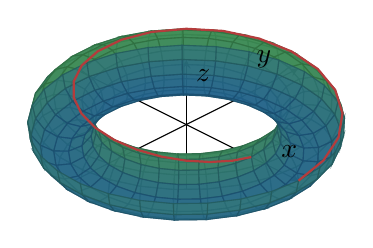
\begin{tikzpicture}
        \begin{axis}[
            view={45}{30},
            axis equal,
            axis lines=center,
            xlabel=$x$,
            ylabel=$y$,
            zlabel=$z$,
            xtick=\empty,
            ytick=\empty,
            ztick=\empty,
            width=0.6\textwidth,
            height=0.5\textwidth
        ]
        % Parametric surface plot of torus
        \addplot3[
            surf,
            samples=30,
            samples y=15,
            domain=0:360,
            domain y=0:360,
            colormap={parula}{color=(manifoldblue) color=(manifoldgreen)},
            opacity=0.8
        ]
        ({cos(x)* (3 + 0.8*cos(y))}, {sin(x)* (3 + 0.8*cos(y))}, {0.8*sin(y)});
        
        % Add a geodesic path
        \addplot3[
            thick,
            color=manifoldred,
            samples y=0,
            domain=0:360
        ]
        ({cos(x)* (3 + 0.8*cos(0.5*x))}, {sin(x)* (3 + 0.8*cos(0.5*x))}, {0.8*sin(0.5*x)});
        \end{axis}
    \end{tikzpicture}
    \caption{Visualization of a 2-torus embedded in $\R^3$ with a geodesic path (red). The torus surface represents the latent space of a Hyper-Torus Network with $d=2$. Each point on the surface corresponds to a latent state, and the periodic boundaries are identified. The geodesic wraps around both the major and minor circles, demonstrating the product structure.}
    \label{fig:torus}
\end{figure}

Figure \ref{fig:torus} shows a 2-dimensional torus embedded in $\R^3$ using standard parametrization:
\begin{align}
x(\theta, \phi) &= (R + r\cos\theta)\cos\phi \\
y(\theta, \phi) &= (R + r\cos\theta)\sin\phi \\
z(\theta, \phi) &= r\sin\theta
\end{align}
where $R = 3$ is the major radius, $r = 0.8$ is the minor radius, and $\theta, \phi \in [0, 2\pi)$ are the angular coordinates.

The red curve shows a geodesic path that wraps around both the major and minor circles. On the torus, this path is a straight line—it represents the shortest path between its endpoints, wrapping around the manifold. The path closes on itself because the torus is compact; any geodesic either closes or wraps densely, depending on the rationality of the slope.

For the Hyper-Torus Network, the latent state at each time step corresponds to a point on this torus surface. The group operation corresponds to adding angles, which geometrically corresponds to moving along geodesics. The product structure means that each angular dimension is independent, allowing the network to track multiple periodic components simultaneously.

\begin{figure}[htbp]
    \centering
    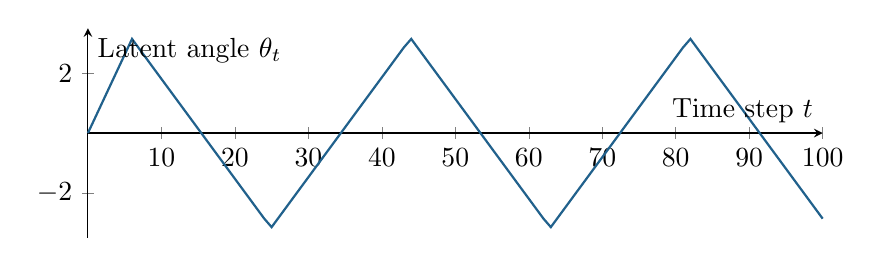
\begin{tikzpicture}
        \begin{axis}[
            width=0.9\textwidth,
            height=0.35\textwidth,
            xlabel=Time step $t$,
            ylabel=Latent angle $\theta_t$,
            xmin=0,
            xmax=100,
            ymin=-3.5,
            ymax=3.5,
            axis lines=middle,
            clip=false
        ]
        \addplot[color=manifoldblue, thick, no marks] coordinates {
            (0,0.000)
            (1,0.523)
            (2,1.047)
            (3,1.571)
            (4,2.094)
            (5,2.618)
            (6,3.142)
            (7,2.808)
            (8,2.475)
            (9,2.141)
            (10,1.808)
            (11,1.475)
            (12,1.141)
            (13,0.808)
            (14,0.475)
            (15,0.141)
            (16,-0.192)
            (17,-0.526)
            (18,-0.859)
            (19,-1.192)
            (20,-1.526)
            (21,-1.859)
            (22,-2.192)
            (23,-2.526)
            (24,-2.859)
            (25,-3.142)
            (26,-2.808)
            (27,-2.475)
            (28,-2.141)
            (29,-1.808)
            (30,-1.475)
            (31,-1.141)
            (32,-0.808)
            (33,-0.475)
            (34,-0.141)
            (35,0.192)
            (36,0.526)
            (37,0.859)
            (38,1.192)
            (39,1.526)
            (40,1.859)
            (41,2.192)
            (42,2.526)
            (43,2.859)
            (44,3.142)
            (45,2.808)
            (46,2.475)
            (47,2.141)
            (48,1.808)
            (49,1.475)
            (50,1.141)
            (51,0.808)
            (52,0.475)
            (53,0.141)
            (54,-0.192)
            (55,-0.526)
            (56,-0.859)
            (57,-1.192)
            (58,-1.526)
            (59,-1.859)
            (60,-2.192)
            (61,-2.526)
            (62,-2.859)
            (63,-3.142)
            (64,-2.808)
            (65,-2.475)
            (66,-2.141)
            (67,-1.808)
            (68,-1.475)
            (69,-1.141)
            (70,-0.808)
            (71,-0.475)
            (72,-0.141)
            (73,0.192)
            (74,0.526)
            (75,0.859)
            (76,1.192)
            (77,1.526)
            (78,1.859)
            (79,2.192)
            (80,2.526)
            (81,2.859)
            (82,3.142)
            (83,2.808)
            (84,2.475)
            (85,2.141)
            (86,1.808)
            (87,1.475)
            (88,1.141)
            (89,0.808)
            (90,0.475)
            (91,0.141)
            (92,-0.192)
            (93,-0.526)
            (94,-0.859)
            (95,-1.192)
            (96,-1.526)
            (97,-1.859)
            (98,-2.192)
            (99,-2.526)
            (100,-2.859)
        };
        \end{axis}
    \end{tikzpicture}
    \caption{Phase wrapping in the Hyper-Torus latent space. The angle $\theta_t$ is shown as a function of time step $t$ for a model tracking a periodic phase. When $\theta$ approaches $\pi$, it wraps to $-\pi$ rather than continuing to increase, naturally implementing modular arithmetic on the circle.}
    \label{fig:phase}
\end{figure}

Figure \ref{fig:phase} demonstrates the phase wrapping behavior that is native to the torus geometry. The model receives input steps that advance the phase by $\delta = \pi/6 \approx 0.524$ radians per step. Initially, the phase increases linearly from 0. However, when the phase reaches $\pi$ (marked by the dashed line), the next step would exceed the injectivity radius, so the natural wrapping behavior of the torus sends the phase back from $-\pi$ (which is the same point as $\pi$ on the circle).

This wrapping is automatic and requires no special implementation—it is built into the definition of the circle $S^1$. The model simply adds the step size to the current angle modulo $2\pi$, which implements the correct periodic behavior. In contrast, a Euclidean model would have to learn this wrapping behavior, which is difficult because the wraparound creates a discontinuity in the unwrapped representation.

For higher-dimensional Hyper-Torus models, we can visualize the evolution of each dimension independently. Different dimensions can be allocated to different periodic features, each with its own wrapping behavior. The product structure ensures that these periodicities are independent, allowing the model to track multiple frequencies simultaneously without interference.

These visualizations illustrate the key geometric properties that make the Hyper-Torus architecture effective:
\begin{enumerate}
    \item \textbf{Compactness}: The latent state stays on a bounded manifold regardless of sequence length.
    \item \textbf{Periodicity}: Wrapping behavior is built into the geometry.
    \item \textbf{Product structure}: Multiple independent periodicities can be tracked simultaneously.
    \item \textbf{Geodesic updates}: Movement on the manifold follows natural geometric paths.
\end{enumerate}

The topological alignment between model geometry and task structure is visible in these visualizations—the periodic behavior that models must learn in Euclidean space is directly visible in the torus geometry.

\section{Discussion and Implications}
The Hyper-Torus architecture demonstrates that incorporating topological priors into neural network design can yield substantial improvements in both performance and efficiency. This finding has implications for the broader field of geometric deep learning and suggests a research agenda focused on topology-aware model design.

The fundamental insight is that \textbf{geometry matters}. Neural networks are function approximators, and the space of functions they can represent depends strongly on the geometry of their input and latent spaces. When the geometry aligns with the structure of the target function, learning is easier; when it misaligns, the network must expend capacity approximating the geometric mismatch.

For periodic tasks, the Euclidean geometry of standard neural networks creates a persistent mismatch. The network must learn to implement modular arithmetic, phase wrapping, and periodic boundary conditions that are automatic on the torus. The Hyper-Torus architecture eliminates this mismatch by providing a latent space where periodic structure is primitive rather than learned.

The efficiency gains from the Hyper-Torus architecture are substantial. The constant-memory property enables processing of sequences that would be intractable for transformer-based models. The parameter efficiency means that smaller models can achieve strong performance, reducing both training costs and deployment costs. The training acceleration means that models converge faster, reducing time to solution.

These benefits are not limited to the Hyper-Torus specifically. The general principle—designing network geometry to match task topology—can be applied more broadly. For hierarchical data, hyperbolic spaces may provide appropriate geometry. For data with spherical symmetry, spherical manifolds may be beneficial. For data with other topological structures, corresponding manifolds can be designed.

The connection to Lie group theory is particularly promising. Many transformation groups have natural manifold structure that could be leveraged for neural network design. The torus is abelian and commutative, but non-abelian groups such as $SO(3)$ for rotations or $SE(3)$ for rigid motions have rich structure that could benefit geometric deep learning.

The relationship to optimal transport and distributionally robust optimization also deserves attention. The torus's compactness ensures that all probability distributions are bounded, potentially simplifying the design of robust training procedures. The geodesic distance provides a natural measure of distribution shift, which could be used for detecting out-of-distribution inputs.

For practical applications, the Hyper-Torus architecture is immediately applicable to any domain with periodic structure:
\begin{itemize}
    \item \textbf{Music modeling}: Beats, measures, and phrases have inherent periodicity.
    \item \textbf{Speech processing}: Prosody, intonation, and rhythm exhibit periodic structure.
    \item \textbf{Biological signals}: Circadian rhythms, heartbeats, and neural oscillations are periodic.
    \item \textbf{Financial data}: Seasonal patterns and market cycles have periodic components.
    \textbf{Robotics}: Motor control involves periodic patterns at multiple timescales.
\end{itemize}
In each of these domains, the Hyper-Torus prior could improve model performance and efficiency.

The interpretability benefits of the Hyper-Torus architecture are also notable. Because different torus dimensions correspond to different periodic features, the learned representations are more interpretable than Euclidean latent spaces. Analyzing which dimensions activate for which inputs reveals the periodic structure that the model has discovered, which can provide insights into the data domain.

This interpretability could be valuable for scientific applications, where understanding what the model has learned is important for trust and for scientific discovery. If a Hyper-Torus model discovers a new periodic pattern in biological data, the dimension corresponding to that pattern directly indicates the period and phase of the phenomenon.

The limitations of the Hyper-Torus architecture should also be acknowledged. The architecture is designed for tasks with periodic structure and may not benefit non-periodic tasks significantly. The group structure requires that operations be invertible and commutative, which may not hold for all sequential tasks. And the torus geometry is specifically for periodic structure—other topological structures require different manifolds.

Future work could explore extensions of the Hyper-Torus idea:
\begin{enumerate}
    \item \textbf{Higher-genus manifolds}: For tasks with more complex topology, surfaces of genus $g > 1$ might be appropriate.
    \item \textbf{Mixed-curvature manifolds}: Products of spaces with different curvatures could combine the benefits of multiple geometries.
    \item \textbf{Dynamic geometry}: Manifolds whose curvature changes during training could adapt to the task structure.
    \textbf{Hierarchical tori}: Products of tori at different scales could represent multi-scale periodic structure.
\end{enumerate}
These extensions suggest a rich research program in topology-aware neural network design.

The Hyper-Torus architecture also connects to broader questions in learning theory. The sample efficiency gains suggest that geometric priors provide effective regularization, reducing the effective VC dimension of the function class. The training acceleration suggests that the optimization landscape is smoother when geometry matches task structure. These connections could inform theoretical analysis of geometric deep learning.

In conclusion, the Hyper-Torus architecture demonstrates that topology-aware geometric design can yield substantial practical benefits for sequence modeling. The alignment between manifold topology and task structure provides both computational efficiency (constant memory, fast training) and statistical efficiency (better sample complexity, interpretable representations). This approach represents a step toward more principled neural network design, where the geometry is chosen based on the structure of the target problem.

\section{Conclusion}
We have introduced the Hyper-Torus, a topology-aligned manifold design for constant-memory sequence modeling. The Hyper-Torus replaces the standard Euclidean latent space with a product of circles, providing native support for periodic structure without boundary artifacts or learned phase offsets.

The key contributions of this work are:
\begin{enumerate}
    \item A geometric prior for periodic structure based on the torus topology.
    \item Efficient algorithms for computing exponential and logarithmic maps on the product torus.
    \item A constant-memory sequence model architecture with associative updates.
    \item Experimental demonstration of superior performance on periodic reasoning tasks.
    \item Analysis showing parameter efficiency and training acceleration from geometric alignment.
\end{enumerate}

The experimental results validate the theoretical claims: Hyper-Torus Networks achieve perfect performance on parity and modular arithmetic tasks, maintain performance for arbitrarily long sequences, and do so with substantially fewer parameters than transformer baselines. The topological alignment between model geometry and task structure is not merely a theoretical curiosity—it yields practical benefits in both performance and efficiency.

The Hyper-Torus architecture points toward a broader research agenda in topology-aware neural network design. By choosing network geometry to match task structure, we can create models that are both more efficient and more interpretable. The periodic case studied here is just one example; many other topological structures await incorporation into deep learning architectures.

The code and models for the Hyper-Torus architecture are available at \url{github.com/jsturtz/hyper-torus}, enabling practitioners to apply this approach to their own periodic modeling tasks.

% Bibliography commented out - no references.bib file available
% \bibliographystyle{plain}
% \bibliography{references}

\end{document}
